\begin{figure*}[t]
\centering
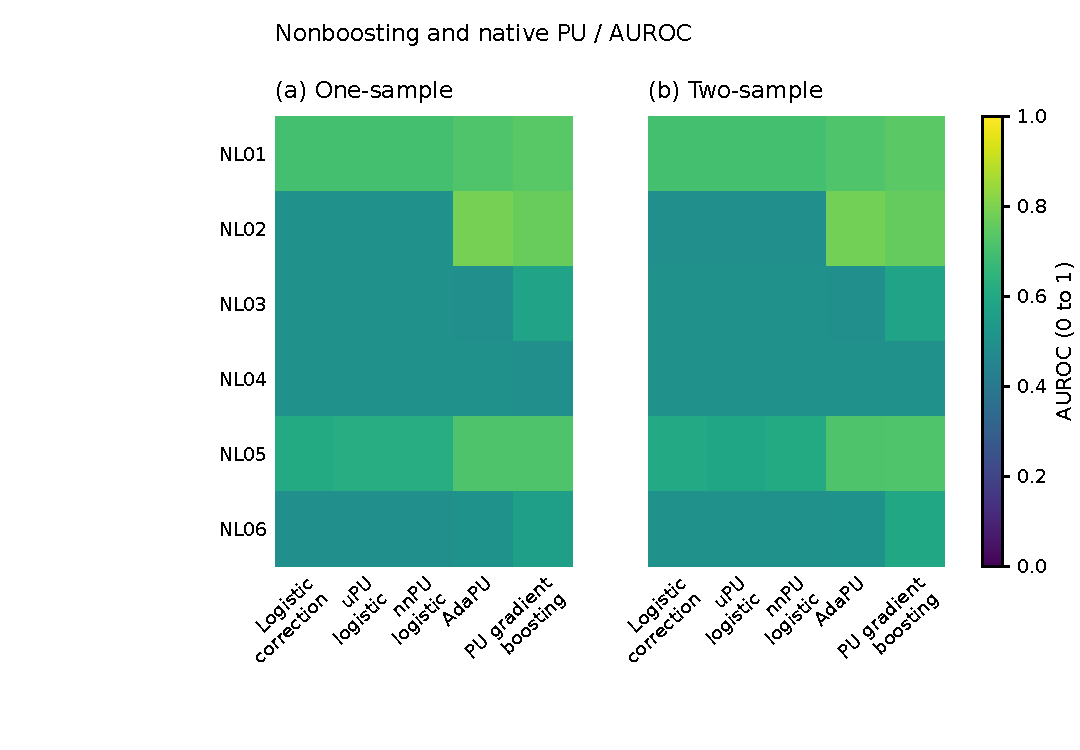
\includegraphics[page=1,width=\textwidth]{mlj_revision/display_package/supplement/figures/fig_s_nonlinear_full.pdf}
\caption{All 25 nonlinear-extension PU configurations, separated into prespecified method blocks. AUROC and AP use final train+validation refits. Individual DGPs are primary, and scales are fixed at 0 to 1. Six unavailable RN refits remain missing; asterisks mark means based on 99 rather than 100 successful refits. Nonboosting and native PU / AUROC. All six nonlinear DGPs. * n=99; all other cells n=100. Missing refits are not imputed.}
\label{fig:fig-s-nonlinear-full-page1}
\end{figure*}

\begin{figure*}[t]
\centering
\includegraphics[page=2,width=\textwidth]{mlj_revision/display_package/supplement/figures/fig_s_nonlinear_full.pdf}
\caption{All 25 nonlinear-extension PU configurations, separated into prespecified method blocks. AUROC and AP use final train+validation refits. Individual DGPs are primary, and scales are fixed at 0 to 1. Six unavailable RN refits remain missing; asterisks mark means based on 99 rather than 100 successful refits. Naive boosting / AUROC. All six nonlinear DGPs. * n=99; all other cells n=100. Missing refits are not imputed.}
\label{fig:fig-s-nonlinear-full-page2}
\end{figure*}

\begin{figure*}[t]
\centering
\includegraphics[page=3,width=\textwidth]{mlj_revision/display_package/supplement/figures/fig_s_nonlinear_full.pdf}
\caption{All 25 nonlinear-extension PU configurations, separated into prespecified method blocks. AUROC and AP use final train+validation refits. Individual DGPs are primary, and scales are fixed at 0 to 1. Six unavailable RN refits remain missing; asterisks mark means based on 99 rather than 100 successful refits. Corrected boosting / AUROC. All six nonlinear DGPs. * n=99; all other cells n=100. Missing refits are not imputed.}
\label{fig:fig-s-nonlinear-full-page3}
\end{figure*}

\begin{figure*}[t]
\centering
\includegraphics[page=4,width=\textwidth]{mlj_revision/display_package/supplement/figures/fig_s_nonlinear_full.pdf}
\caption{All 25 nonlinear-extension PU configurations, separated into prespecified method blocks. AUROC and AP use final train+validation refits. Individual DGPs are primary, and scales are fixed at 0 to 1. Six unavailable RN refits remain missing; asterisks mark means based on 99 rather than 100 successful refits. RN boosting / AUROC. All six nonlinear DGPs. * n=99; all other cells n=100. Missing refits are not imputed.}
\label{fig:fig-s-nonlinear-full-page4}
\end{figure*}

\begin{figure*}[t]
\centering
\includegraphics[page=5,width=\textwidth]{mlj_revision/display_package/supplement/figures/fig_s_nonlinear_full.pdf}
\caption{All 25 nonlinear-extension PU configurations, separated into prespecified method blocks. AUROC and AP use final train+validation refits. Individual DGPs are primary, and scales are fixed at 0 to 1. Six unavailable RN refits remain missing; asterisks mark means based on 99 rather than 100 successful refits. CS boosting / AUROC. All six nonlinear DGPs. * n=99; all other cells n=100. Missing refits are not imputed.}
\label{fig:fig-s-nonlinear-full-page5}
\end{figure*}

\begin{figure*}[t]
\centering
\includegraphics[page=6,width=\textwidth]{mlj_revision/display_package/supplement/figures/fig_s_nonlinear_full.pdf}
\caption{All 25 nonlinear-extension PU configurations, separated into prespecified method blocks. AUROC and AP use final train+validation refits. Individual DGPs are primary, and scales are fixed at 0 to 1. Six unavailable RN refits remain missing; asterisks mark means based on 99 rather than 100 successful refits. Nonboosting and native PU / AP. All six nonlinear DGPs. * n=99; all other cells n=100. Missing refits are not imputed.}
\label{fig:fig-s-nonlinear-full-page6}
\end{figure*}

\begin{figure*}[t]
\centering
\includegraphics[page=7,width=\textwidth]{mlj_revision/display_package/supplement/figures/fig_s_nonlinear_full.pdf}
\caption{All 25 nonlinear-extension PU configurations, separated into prespecified method blocks. AUROC and AP use final train+validation refits. Individual DGPs are primary, and scales are fixed at 0 to 1. Six unavailable RN refits remain missing; asterisks mark means based on 99 rather than 100 successful refits. Naive boosting / AP. All six nonlinear DGPs. * n=99; all other cells n=100. Missing refits are not imputed.}
\label{fig:fig-s-nonlinear-full-page7}
\end{figure*}

\begin{figure*}[t]
\centering
\includegraphics[page=8,width=\textwidth]{mlj_revision/display_package/supplement/figures/fig_s_nonlinear_full.pdf}
\caption{All 25 nonlinear-extension PU configurations, separated into prespecified method blocks. AUROC and AP use final train+validation refits. Individual DGPs are primary, and scales are fixed at 0 to 1. Six unavailable RN refits remain missing; asterisks mark means based on 99 rather than 100 successful refits. Corrected boosting / AP. All six nonlinear DGPs. * n=99; all other cells n=100. Missing refits are not imputed.}
\label{fig:fig-s-nonlinear-full-page8}
\end{figure*}

\begin{figure*}[t]
\centering
\includegraphics[page=9,width=\textwidth]{mlj_revision/display_package/supplement/figures/fig_s_nonlinear_full.pdf}
\caption{All 25 nonlinear-extension PU configurations, separated into prespecified method blocks. AUROC and AP use final train+validation refits. Individual DGPs are primary, and scales are fixed at 0 to 1. Six unavailable RN refits remain missing; asterisks mark means based on 99 rather than 100 successful refits. RN boosting / AP. All six nonlinear DGPs. * n=99; all other cells n=100. Missing refits are not imputed.}
\label{fig:fig-s-nonlinear-full-page9}
\end{figure*}

\begin{figure*}[t]
\centering
\includegraphics[page=10,width=\textwidth]{mlj_revision/display_package/supplement/figures/fig_s_nonlinear_full.pdf}
\caption{All 25 nonlinear-extension PU configurations, separated into prespecified method blocks. AUROC and AP use final train+validation refits. Individual DGPs are primary, and scales are fixed at 0 to 1. Six unavailable RN refits remain missing; asterisks mark means based on 99 rather than 100 successful refits. CS boosting / AP. All six nonlinear DGPs. * n=99; all other cells n=100. Missing refits are not imputed.}
\label{fig:fig-s-nonlinear-full-page10}
\end{figure*}
